% Options for packages loaded elsewhere
\PassOptionsToPackage{unicode}{hyperref}
\PassOptionsToPackage{hyphens}{url}
\PassOptionsToPackage{dvipsnames,svgnames,x11names}{xcolor}
%
\documentclass[
  10pt,
  a4paperpaper,
  DIV=11,
  numbers=noendperiod,
  oneside]{scrreprt}

\usepackage{amsmath,amssymb}
\usepackage{iftex}
\ifPDFTeX
  \usepackage[T1]{fontenc}
  \usepackage[utf8]{inputenc}
  \usepackage{textcomp} % provide euro and other symbols
\else % if luatex or xetex
  \usepackage{unicode-math}
  \defaultfontfeatures{Scale=MatchLowercase}
  \defaultfontfeatures[\rmfamily]{Ligatures=TeX,Scale=1}
\fi
\usepackage{lmodern}
\ifPDFTeX\else  
    % xetex/luatex font selection
\fi
% Use upquote if available, for straight quotes in verbatim environments
\IfFileExists{upquote.sty}{\usepackage{upquote}}{}
\IfFileExists{microtype.sty}{% use microtype if available
  \usepackage[]{microtype}
  \UseMicrotypeSet[protrusion]{basicmath} % disable protrusion for tt fonts
}{}
\makeatletter
\@ifundefined{KOMAClassName}{% if non-KOMA class
  \IfFileExists{parskip.sty}{%
    \usepackage{parskip}
  }{% else
    \setlength{\parindent}{0pt}
    \setlength{\parskip}{6pt plus 2pt minus 1pt}}
}{% if KOMA class
  \KOMAoptions{parskip=half}}
\makeatother
\usepackage{xcolor}
\usepackage[top=25mm,bottom=25mm,left=17.5mm,right=82.5mm,marginparsep=10mm,marginparwidth=55mm]{geometry}
\setlength{\emergencystretch}{3em} % prevent overfull lines
\setcounter{secnumdepth}{5}
% Make \paragraph and \subparagraph free-standing
\makeatletter
\ifx\paragraph\undefined\else
  \let\oldparagraph\paragraph
  \renewcommand{\paragraph}{
    \@ifstar
      \xxxParagraphStar
      \xxxParagraphNoStar
  }
  \newcommand{\xxxParagraphStar}[1]{\oldparagraph*{#1}\mbox{}}
  \newcommand{\xxxParagraphNoStar}[1]{\oldparagraph{#1}\mbox{}}
\fi
\ifx\subparagraph\undefined\else
  \let\oldsubparagraph\subparagraph
  \renewcommand{\subparagraph}{
    \@ifstar
      \xxxSubParagraphStar
      \xxxSubParagraphNoStar
  }
  \newcommand{\xxxSubParagraphStar}[1]{\oldsubparagraph*{#1}\mbox{}}
  \newcommand{\xxxSubParagraphNoStar}[1]{\oldsubparagraph{#1}\mbox{}}
\fi
\makeatother


\providecommand{\tightlist}{%
  \setlength{\itemsep}{0pt}\setlength{\parskip}{0pt}}\usepackage{longtable,booktabs,array}
\usepackage{calc} % for calculating minipage widths
% Correct order of tables after \paragraph or \subparagraph
\usepackage{etoolbox}
\makeatletter
\patchcmd\longtable{\par}{\if@noskipsec\mbox{}\fi\par}{}{}
\makeatother
% Allow footnotes in longtable head/foot
\IfFileExists{footnotehyper.sty}{\usepackage{footnotehyper}}{\usepackage{footnote}}
\makesavenoteenv{longtable}
\usepackage{graphicx}
\makeatletter
\def\maxwidth{\ifdim\Gin@nat@width>\linewidth\linewidth\else\Gin@nat@width\fi}
\def\maxheight{\ifdim\Gin@nat@height>\textheight\textheight\else\Gin@nat@height\fi}
\makeatother
% Scale images if necessary, so that they will not overflow the page
% margins by default, and it is still possible to overwrite the defaults
% using explicit options in \includegraphics[width, height, ...]{}
\setkeys{Gin}{width=\maxwidth,height=\maxheight,keepaspectratio}
% Set default figure placement to htbp
\makeatletter
\def\fps@figure{htbp}
\makeatother

\usepackage{booktabs}
\usepackage[scaled=0.98, sups]{XCharter}
\usepackage[scaled=1.04, varqu, varl]{inconsolata}
\usepackage[type1]{cabin}
\usepackage{algorithm}
\usepackage{algpseudocode}
\usepackage{array}
\usepackage{multirow}
\usepackage{tikz}
\usepackage{framed}
\usepackage{mdframed}
%\usepackage[xcharter, vvarbb, scaled=1.07]{newtxmath}
\usepackage{xcolor}
\definecolor{CodeBackground}{HTML}{F0F0F0}
\definecolor{CodeString}{HTML}{008080}
\definecolor{CodeComment}{HTML}{008000}
\usepackage{layout}

\usepackage{fvextra}
\DefineVerbatimEnvironment{Highlighting}{Verbatim}{breaklines,commandchars=\\\{\}}

\newenvironment{cntrlplcy}{}{}

\def\fps@table{htbp}
\usepackage{listings}
\lstset{breaklines=true, columns=flexible, aboveskip=-8pt, belowskip=-10pt, showlines}
\lstdefinelanguage{CMPseudo}{%
  language     = Python,
  morekeywords = {zeros, TRANSITION, TRIGGER, WITH, SCHEDULE, TIME, FOR, IN, WITH, IF, THEN, END, IS, NOT, empty, START, CREATE},
  numbers=left,
  numberstyle=\footnotesize,
  basicstyle = \small \ttfamily,
  keywordstyle = \color{blue},
  stringstyle = \color{CodeString},
  commentstyle=\color{CodeComment},
  showstringspaces = false,
  backgroundcolor=\color{CodeBackground},
}

\lstdefinelanguage{JavaNew}{%
  language     = Java,
  numbers=left,
  numberstyle=\footnotesize,
  backgroundcolor=\color{CodeBackground},
  keywordstyle = \color{blue},
  basicstyle = \small \ttfamily
}

\newlength{\lastcol}

\setcounter{topnumber}{8}
\setcounter{bottomnumber}{8}
\setcounter{totalnumber}{8}

% \pagestyle{myheadings}
% \markright{\rightmark}

\renewcommand*{\partpagestyle}{empty}

\newmdenv[hidealllines=true, innerleftmargin=0cm, innerrightmargin=0cm, innertopmargin=0cm, innerbottommargin=0cm]{codebox}

\newmdenv[nobreak=false, hidealllines=true, backgroundcolor=CodeBackground]{codeout}

\KOMAoption{captions}{tableheading}
\makeatletter
\@ifpackageloaded{float}{}{\usepackage{float}}
\floatstyle{plain}
\@ifundefined{c@chapter}{\newfloat{cntrlplcy}{h}{locntrlplcy}}{\newfloat{cntrlplcy}{h}{locntrlplcy}[chapter]}
\floatname{cntrlplcy}{Control Policy}
\newcommand*\listofcntrlplcys{\listof{cntrlplcy}{List of Control Policys}}
\makeatother
\makeatletter
\@ifpackageloaded{bookmark}{}{\usepackage{bookmark}}
\makeatother
\makeatletter
\@ifpackageloaded{caption}{}{\usepackage{caption}}
\AtBeginDocument{%
\ifdefined\contentsname
  \renewcommand*\contentsname{Table of contents}
\else
  \newcommand\contentsname{Table of contents}
\fi
\ifdefined\listfigurename
  \renewcommand*\listfigurename{List of Figures}
\else
  \newcommand\listfigurename{List of Figures}
\fi
\ifdefined\listtablename
  \renewcommand*\listtablename{List of Tables}
\else
  \newcommand\listtablename{List of Tables}
\fi
\ifdefined\figurename
  \renewcommand*\figurename{Figure}
\else
  \newcommand\figurename{Figure}
\fi
\ifdefined\tablename
  \renewcommand*\tablename{Table}
\else
  \newcommand\tablename{Table}
\fi
}
\@ifpackageloaded{float}{}{\usepackage{float}}
\floatstyle{ruled}
\@ifundefined{c@chapter}{\newfloat{codelisting}{h}{lop}}{\newfloat{codelisting}{h}{lop}[chapter]}
\floatname{codelisting}{Listing}
\newcommand*\listoflistings{\listof{codelisting}{List of Listings}}
\makeatother
\makeatletter
\makeatother
\makeatletter
\@ifpackageloaded{caption}{}{\usepackage{caption}}
\@ifpackageloaded{subcaption}{}{\usepackage{subcaption}}
\makeatother
\makeatletter
\@ifpackageloaded{sidenotes}{}{\usepackage{sidenotes}}
\@ifpackageloaded{marginnote}{}{\usepackage{marginnote}}
\makeatother

\ifLuaTeX
  \usepackage{selnolig}  % disable illegal ligatures
\fi
\usepackage{bookmark}

\IfFileExists{xurl.sty}{\usepackage{xurl}}{} % add URL line breaks if available
\urlstyle{same} % disable monospaced font for URLs
\hypersetup{
  pdftitle={ENGSCI 355 Labs},
  pdfauthor={Thomas Adams},
  colorlinks=true,
  linkcolor={blue},
  filecolor={Maroon},
  citecolor={Blue},
  urlcolor={Blue},
  pdfcreator={LaTeX via pandoc}}


\title{ENGSCI 355 Labs}
\author{Thomas Adams}
\date{2024-08-29}

\begin{document}
\maketitle

\renewcommand*\contentsname{Table of contents}
{
\hypersetup{linkcolor=}
\setcounter{tocdepth}{2}
\tableofcontents
}

\bookmarksetup{startatroot}

\chapter*{Preface}\label{preface}
\addcontentsline{toc}{chapter}{Preface}

\markboth{Preface}{Preface}

These are an online version of the Labs for ENGSCI 355. The topics
covered are: a hands-on simulation of a manufacturing process;
conceptual modelling using HCCM; implementing HCCM models in Jaamsim;
and missing data imputaton.

\part{Practical Lab}

\chapter{Operations System in Practice}\label{sec-hands-on-sim}

The goal of this lab is to give you some hands-on experience with an
operations system, the type of system that we will be focussing on
simulating. Hopefully this will give you some idea of what is needed to
simulate a system in terms of:

\begin{itemize}
\tightlist
\item
  the components of the system and how they interact with each other
  (entities and their behaviour);
\item
  the type and amount of information/data that is needed, both for
  activity durations and control policies;
\item
  the types of experiments that can be performed and how the system can
  be redesigned.
\end{itemize}

\section{Making Paper Cars}\label{making-paper-cars}

The system that we will use as an example is making a car out of paper.
You will each be given a piece of paper with the net of paper car on it
as in Figure~\ref{fig-car_net}.

\begin{marginfigure}

\centering{

\includegraphics{chapters/hands_on_production/figures/Car_Net_Blank.png}

}

\caption{\label{fig-car_net}The Net Used to Make Paper Cars}

\end{marginfigure}%

You will also get a pair of scissors, some tape, and blank pieces of
paper. To make the car:

\begin{enumerate}
\def\labelenumi{\arabic{enumi}.}
\tightlist
\item
  Trace the net onto a new piece of paper.
\item
  Cut the new net out.
\item
  Fold the paper and tape the edges shut placing the tabs on the inside.
\end{enumerate}

Figure~\ref{fig-car_complete} shows an example of a completed car.

\begin{marginfigure}

\centering{

\includegraphics{chapters/hands_on_production/figures/Car_Complete.jpg}

}

\caption{\label{fig-car_complete}A Completed Car}

\end{marginfigure}%

First everyone should make one car by themselves. Once you have, show
one of the instructors to get signed off. Then, discuss with you group
how you can work together to make paper cars. You might want to
experiment with different setups/policies and try making a few cars to
see how long it takes and gather some data.

There will be a competition to see which group can make the most cars in
10 minutes. Before the time starts each group must submit an estimate of
how many cars they believe they will be able to make. The score for each
group will then be comprised of the following elements:

\begin{itemize}
\tightlist
\item
  1 point for each car completed up to and including the estimated
  number.
\item
  0.25 points for each car completed above the estimated number.
\item
  -0.75 points for each car not completed in the estimated number.
\end{itemize}

Additionally, the following rules must be followed:

\begin{enumerate}
\def\labelenumi{\arabic{enumi}.}
\tightlist
\item
  Each car must be traced and cut individually.
\item
  Cars must be the same shape as the original template, including tabs.
\item
  You can have as many stencils as you like.
\item
  All final cars must have started as a blank, unfolded piece of paper.
\item
  You may not have any pre-cut tape or nets.
\item
  All cars must have been made only by members of your group.
\item
  All cars must be folded and taped neatly to count. The lecturer has
  final say on whether a car meets the required neatness.
\end{enumerate}

\section{Reflections}\label{reflections}

Now that you have attempted to make as many cars as you can you may wish
to reflect on the process by asking yourself the following questions:

\begin{itemize}
\tightlist
\item
  Did your group have any traced/cut out cars left at the end?
\item
  What was the bottleneck/slowest part of the system?
\item
  Did you collect any data/do any experiments? If so, did they help?
  Would you do more/different ones now?
\item
  What would you do differently next time?
\end{itemize}

The process that we considered was relatively simple. Cinsider how would
your group's strategy change if any of the following additional
conditions were added:

\begin{itemize}
\tightlist
\item
  Blank pieces of paper for you to trace onto only become available one
  at a time every two minutes;
\item
  You have to make different styles of cars on demand;
\item
  There is a limit to how many traced nets/cut pieces of tape you can
  have at any point (buffer limit);
\item
  Each time a pair of scissors is stopped being used there is a cooldown
  time of 1 minute.
\end{itemize}

\part{Conceptual Modelling Labs}

\chapter{HCCM Framework}\label{hccm-framework}

This chapter describes the Hierarchical Control Conceptual Modelling
(HCCM) framework which is used to build a conceptual model, aligned with
the HCCM standard from lectures, that represents the practical activity,
i.e., making paper cars, from Chapter~\ref{sec-hands-on-sim}.

Working in the same groups as for the practical activity and using this
chapter as guidance, over the next two labs you will work through the
phases for HCCM modelling shown in Figure~\ref{fig-cm_phases} and
complete templates for those steps. In the next lab you will complete
phases 1, 2, 3, and start phase 4. The remainder of phase 4 will be
completed in the lab after that. Chapter~\ref{sec-hands-on-sim} provides
a partially completed conceptual model of the car making system that you
can use as a starting point.

\begin{figure*}[htbp]

\centering{

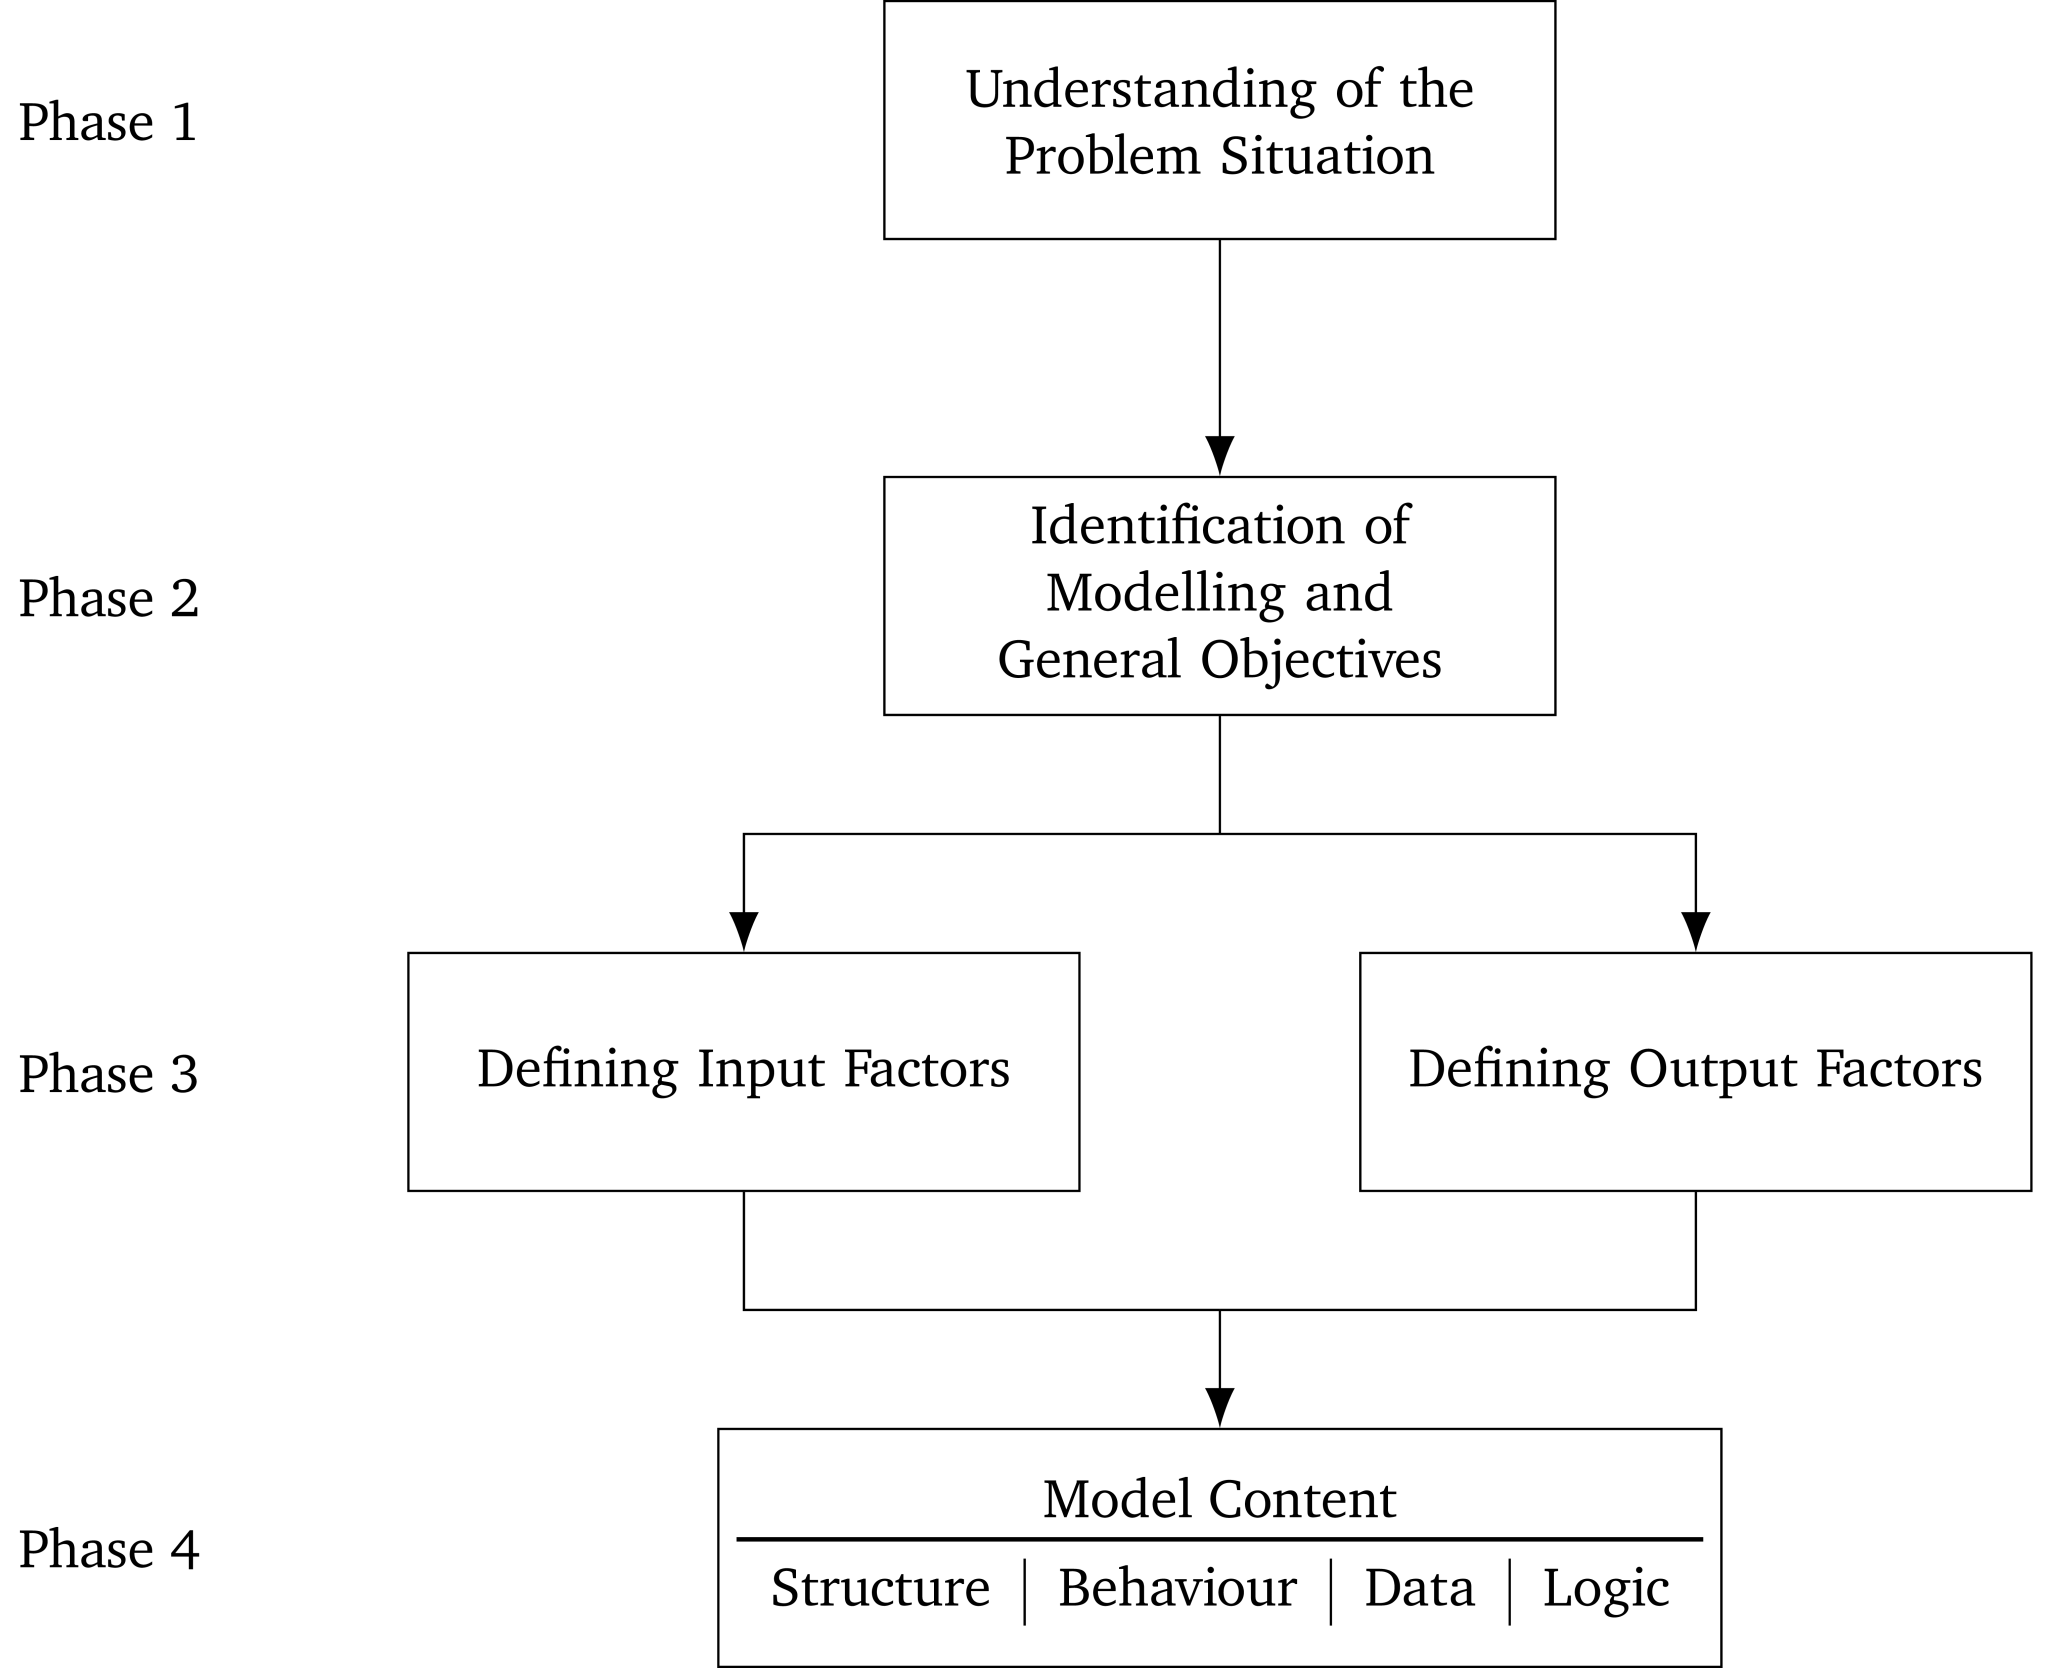
\includegraphics[width=129mm,height=\textheight]{chapters/hccm_framework/figures/cm_phases.pdf}

}

\caption{\label{fig-cm_phases}Conceptual Modelling Phases}

\end{figure*}%

\section{Understanding of the Problem
Situation}\label{understanding-of-the-problem-situation}

In Phase 1, in order to understand the problem situation, you need to
summarise what is happening in a concise way. There is no strict rule
for the best way to do this. One good approach is listening to the
problem ``holder'', i.e., person/people who have the problem such as a
client, then reflecting what you have heard in a couple of paragraphs
with lists of key details and questions. You can then work through one
or more iterations of feedback and refinement to get a final, agreed
upon problem description.

\section{Identification of Modelling and General
Objectives}\label{identification-of-modelling-and-general-objectives}

For Phase 2, as described in lectures, there are two types of objectives
to consider when developing a simulation:

\begin{quote}
``The second step deals with the determination of the objectives.
According to Robinson {[}26{]} they drive all aspects of the modeling
process and are a subset of an organization's aims. Further, objectives
can be classified into modeling and general objectives, where the latter
are concerned with the flexibility, run-speed, visual-display and
model/component reuse.''
\end{quote}

For the modelling objective you may like to think about what you trying
to discover using simulation, and what level of performance you are
trying to achieve in which areas/metrics.

\section{Defining Output Responses}\label{defining-output-responses}

Phase 3 includes defining both the output responses and input factors.
You can do these in either order, but it can often be useful to define
the output responses first, as it may help you think about what inputs
will influence the outputs.

Output responses are things that can be measured and compared to
understand how a system has behaved/performed. They are the metrics used
to compare different simulation scenarios. The output responses should
let you know whether the modelling objectives have been achieved and why
or how. You may also want to consider how this will be reported (tables,
graphs, etc.).

\section{Defining Input Factors}\label{defining-input-factors}

Input factors are things that can be changed and may modify how a system
behaves/performs. They are often defined to create multiple different
scenarios to compare via simulation. They are also what you can change
to try and achieve the modelling objectives.

\section{Model Content}\label{model-content}

In Phase 4 the model content is defined. There is no strict order in
which you need to complete the four components (structre, behaviour,
data, and logic). A possible approach, that we will take in this lab, is
to:

\begin{enumerate}
\def\labelenumi{\arabic{enumi}.}
\tightlist
\item
  Identify the entities;
\item
  Draw the behavioural paths;
\item
  Define the data;
\item
  Define the structure (including the entities again);
\item
  Define the logic.
\end{enumerate}

Using this approach you may still find yourself deciding to add/remove
parts that you have already defined. This is a normal part of the
conceptual modelling process, and you need to go back to the part of the
process you want to change -- for example adding and entity or activity
-- and then update the rest of the CM.

For the model content definition of our conceptual model we will follow
the new HCCM standard. This standard is presented in an academic article
(currently under review) that is available on Canvas under
\texttt{Files > Lectures > Conceptual Modelling} in the file
\href{https://canvas.auckland.ac.nz/courses/113292/files/folder/Lectures/Conceptual\%20Modelling?preview=12376819}{hccm-standard.pdf}

\subsection{Identifying Entities}\label{identifying-entities}

Before formally defining entities it is often useful to identify
entities in the system and whether they are active, i.e., have behaviour
like a doctor or patient, or passive, i.e., are part of the system that
should be modelled but that don't have explicit behaviour like a waiting
room with a given capacity, but that doesn't actually have defined
actions.

The goal is to identify everything that is involved in a meaningful way
in all of the activities that are important to the system. Thinking
about the inputs and outputs can also be useful. Clearly the entities
must be influenced in some way by the inputs, and they must themselves
influence the outputs. You may also consider that an activity does not
have a significant influence on the performance of the system, and
decide to exclude it -- and therefore any entities that are involved
only in that activity. Likewise the participation of a particular entity
in an activity might be deemed inconsequential and therefore excluded.
Although it is possible to revisit and add/remove entities later, at
this stage you want to consider the whole system carefully, as it is
easier to include/exclude an entity now than to change it later.

\subsection{Drawing Behavioural Paths}\label{drawing-behavioural-paths}

Once preliminary identification of entities has been done, behavioural
paths for each of the active entities should be drawn. These are
essentially flowcharts with a special structure. Circles represent
events, usually used when entities are arriving and leaving. Rectangles
represent activities, including when entities have to wait for another
activity. Red squares at the top left of an activity (or sometimes an
event) let us know that some logic is triggered when the activity
starts. This generally occurs at the start of ``wait'' activities and is
used to check whether the conditions that mean the entity can stop
waiting and move on to the next activity are met.

What we are trying to do when drawing the behavioural paths is identify
the activities and events that the entities participate in, the possible
orders that these can occur in, and any points where some control logic
needs to be used.

Both when identifying the entities and drawing the behavioural paths it
is important to keep track of any assumptions and simplifications that
you make.

\subsection{Define the Data}\label{define-the-data}

The data for the conceptual model includes both variables, and data
modules. Variables can change their value throughout the simulation and
are generally used to store some information temporarily before it is
required later in the simulation. Data modules contain the information
that is needed to perform the simulation and can be collected
beforehand. Data mocules can also represent the input/experimental
factors -- the things that may change between different simulation
scenarios. For each data module the following information should be
given:

\begin{enumerate}
\def\labelenumi{\arabic{enumi}.}
\tightlist
\item
  The name of the data module;
\item
  The source of the data, where the information was obtained;
\item
  The way the data is modelled, is it represented by a constant, a
  distribution, etc.
\item
  Whether the output is deterministic or stochastic;
\item
  The inputs that the module requires;
\item
  The quantity that the module outputs.
\end{enumerate}

When presenting a conceptual model is useful to put the data first, as
it is often referenced throughout the rest of the conceptual model.

\subsection{Define the Structure}\label{define-the-structure}

To define the structure we start with formally defining the entities by
listing them along with any attributes that they have. Some common
attributes, such as ID number and the activity that the entity is
currently participating in, are often omitted to avoid repitition.
Attributes are usually included either to assist with the system
behaviour -- for example record whether a patient has had a test -- or
to capture the perfomance of the system -- how long something has waited
for.

Next we define the transitions. Each arrow on a behavioural diagram
corresponds to a transition. We can collate these in a table describing:
the entity that is performing the transition, and the events that the
entity transitions from and to. You can simply number them starting from
1, or adopt a convention of using the entity's initial as a prefix.

Once the transitions have been defined we can define the activities and
events. Usually these are presented in two tables, one for the
activities and one for the events. For each event (either standalone or
as part of an activity) the table should include:

\begin{enumerate}
\def\labelenumi{\arabic{enumi}.}
\tightlist
\item
  The participant(s);
\item
  The type -- either scheduled or controlled;
\item
  The state changes that occur when the event happens.
\end{enumerate}

The main things that occur in state changes are:

\begin{itemize}
\tightlist
\item
  Schedule an end event -- usually in the start event of an activity
  with a scheduled end event;
\item
  Starting another activity/event -- this usually happens in a scheduled
  end event where an entity is transitioning to another scheduled event;
\item
  Trigger some logic -- often in the start event of an activity with a
  controlled end event.
\end{itemize}

The simulation start event, and arrive events are often more complicated
and involve scheduling the initial events and creating entities.

\subsection{Define the Logic}\label{define-the-logic}

The final part of the conceptual model content is the logic. Each
trigger that you drew in a behvioural path (the red squares) should
correspond first to a trigger statement in the state changes of an
event, and a piece of logic defined here. These pieces of logic are used
to determine how the system behaves -- what activity an entity should do
next. It is common to have logic control the behaviour when one entity
needs to wait for another, as when the first entity arrives it needs to
check whether the other is free to perform an activity with it. The
logic is usually presented as pseudocode, alongside the entity that
triggers the logic.

\section{Assumptions and
Simplifications}\label{assumptions-and-simplifications}

Throughout the four phases of the HCCM framework you should document the
assumptions and simplifications that you make. Assumptions are related
to uncertainties about the system being modelled, and are used to fill
in gaps in the information that is required for the simulation.
Simplifications are changes that are made to the model to make it easier
to defined or implement.

\chapter{Inputs, Outputs, and
Behaviour}\label{inputs-outputs-and-behaviour}

In this lab you will complete the first three Phases of the HCCM
framework, and part of the fourth, with your group.

\section{Understanding of the Problem
Situation}\label{understanding-of-the-problem-situation-1}

In the box below write a problem description for making paper cars,
think about what you are trying to solve/discover by simulating this
activity. You may want to look at Chapter~\ref{sec-hands-on-sim} again
to remind yourself about the process.

\begin{figure*}

\begin{mdframed}[innerbottommargin=3cm]

~

~

~

~

~

~

~

~

\end{mdframed}

\end{figure*}%

\section{Modelling Objectives}\label{modelling-objectives}

In the box below write the modelling objectives for making paper cars,
i.e., what are you trying to discover using simulation?

\begin{figure*}

\begin{mdframed}[innerbottommargin=3cm]

~

~

~

~

~

~

~

~

\end{mdframed}

\end{figure*}%

\newpage{}

\section{General Objectives}\label{general-objectives}

In the box below write the general objectives for making paper cars,
i.e., what are some of the general properties you'd like your simulation
to have?

\begin{figure*}

\begin{mdframed}[innerbottommargin=4.5cm]

~

~

~

~

~

~

~

~

~

~

\end{mdframed}

\end{figure*}%

\section{Defining Output Responses}\label{defining-output-responses-1}

In the box below write the output responses for making paper cars, i.e.,
what are you going to measure to determine the performance of the
system?

\begin{figure*}

\begin{mdframed}[innerbottommargin=4.5cm]

~

~

~

~

~

~

~

~

~

~

\end{mdframed}

\end{figure*}%

\newpage{}

\section{Defining Input Factors}\label{defining-input-factors-1}

In the box below write the input factors for making paper cars, i.e.,
what are you going to change to achieve the modelling objectives?

\begin{figure*}

\begin{mdframed}[innerbottommargin=4.5cm]

~

~

~

~

~

~

~

~

~

~

\end{mdframed}

\end{figure*}%

\section{Identifying Entities}\label{identifying-entities-1}

In the box below list the entities for making paper cars.

\begin{figure*}

\begin{mdframed}[innerbottommargin=4.5cm]

~

~

~

~

~

~

~

~

~

~

\end{mdframed}

\end{figure*}%

\newpage{}

\section{Drawing Behavioural Paths}\label{drawing-behavioural-paths-1}

The activity diagrams for the pencil \& template, and scissors are given
below in Figures~\ref{fig-pencil_act}, and~\ref{fig-scissors_act}.

\begin{figure}[htbp]

\centering{

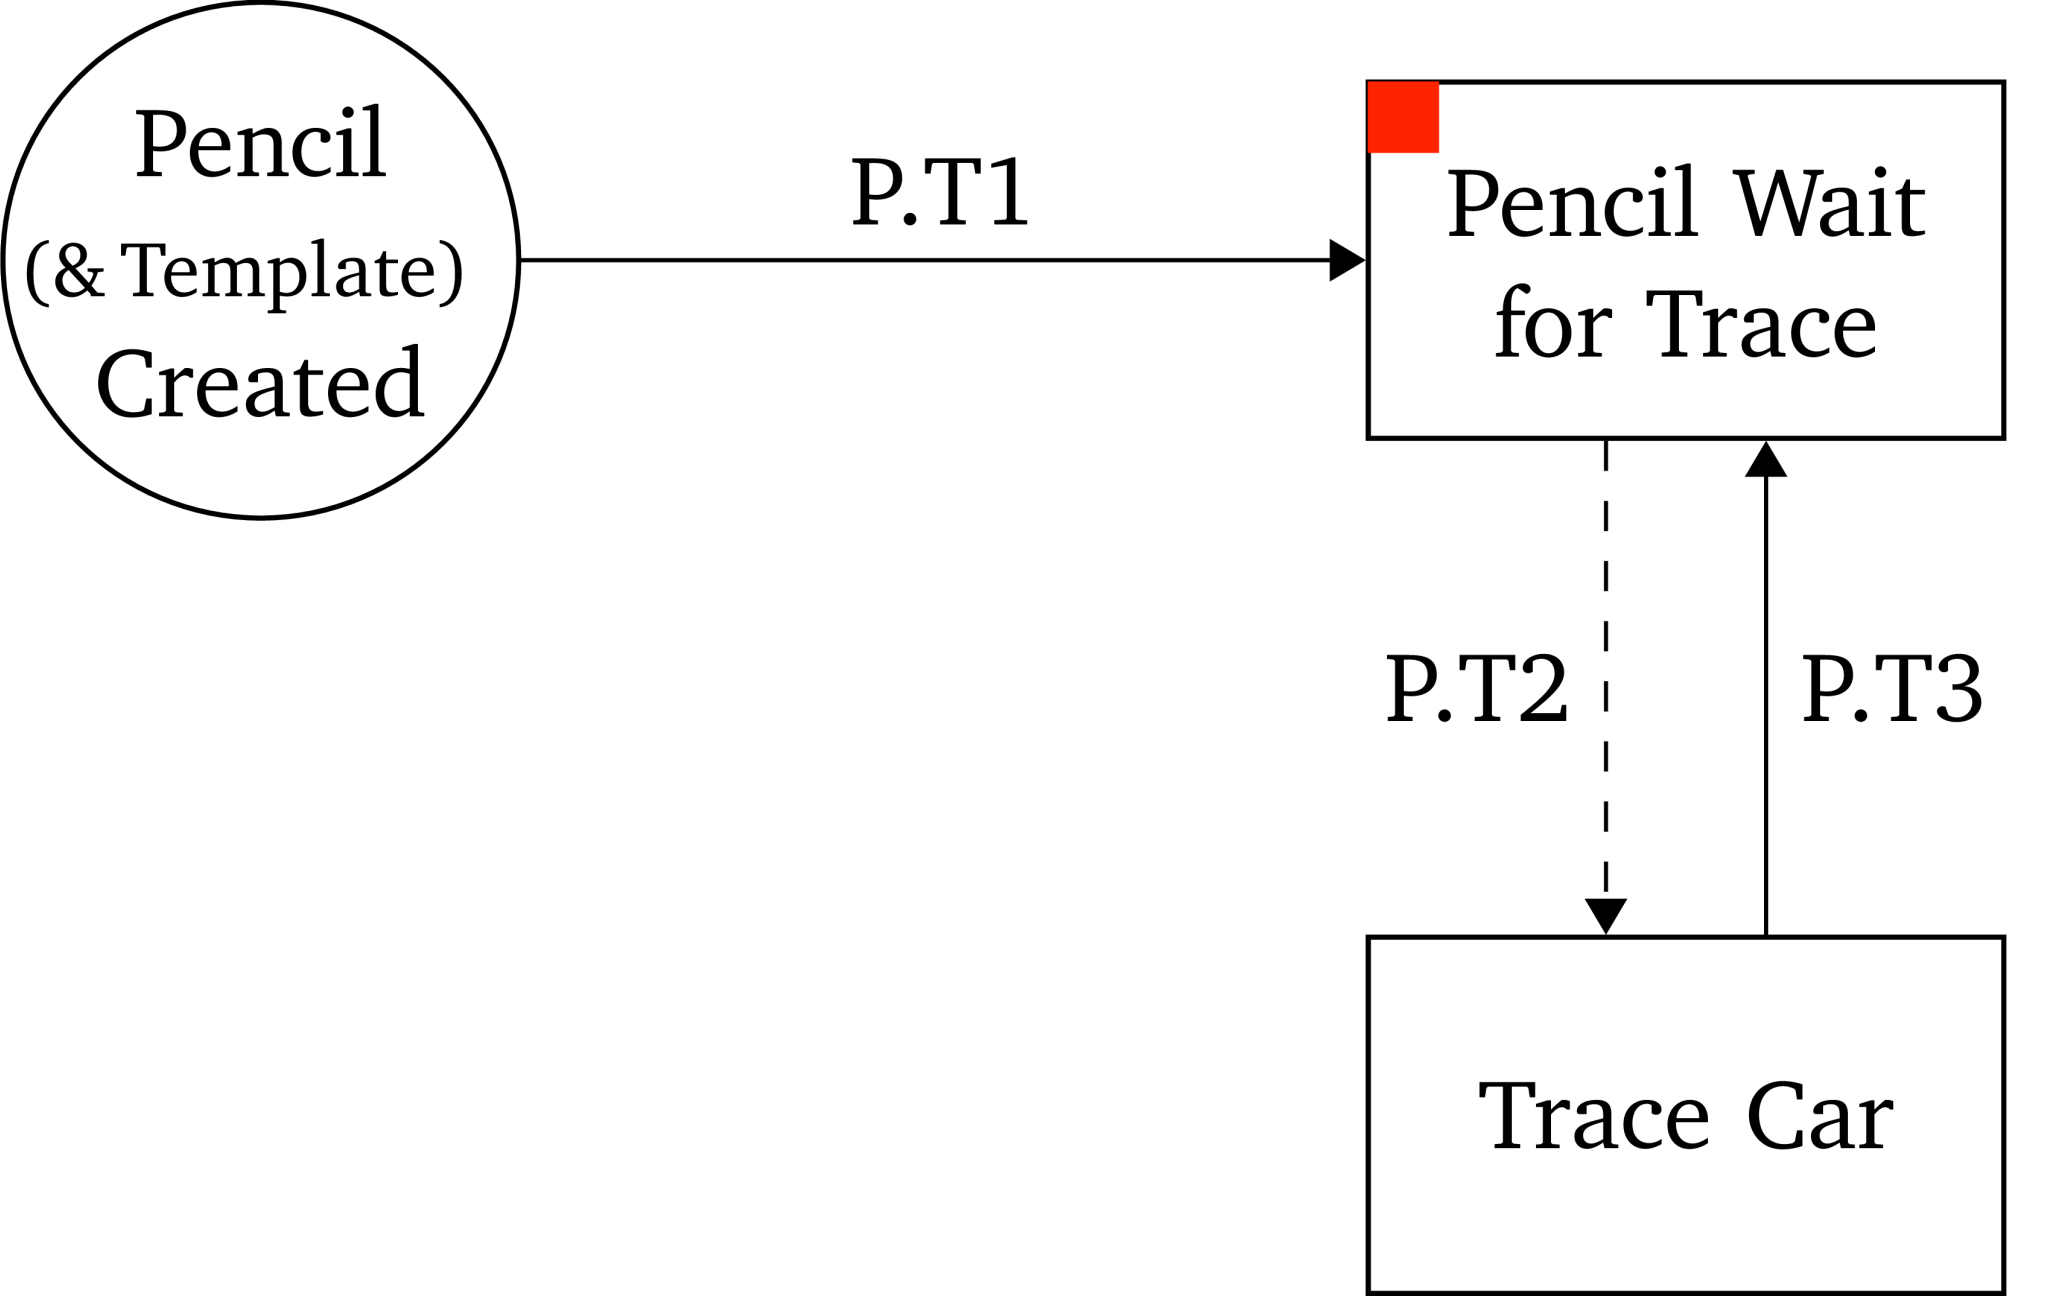
\includegraphics[width=72mm,height=\textheight]{chapters/cm_io_behaviour/figures/pencil-activity.pdf}

}

\caption{\label{fig-pencil_act}Pencil Activity Diagram}

\end{figure}%

\begin{figure}[htbp]

\centering{

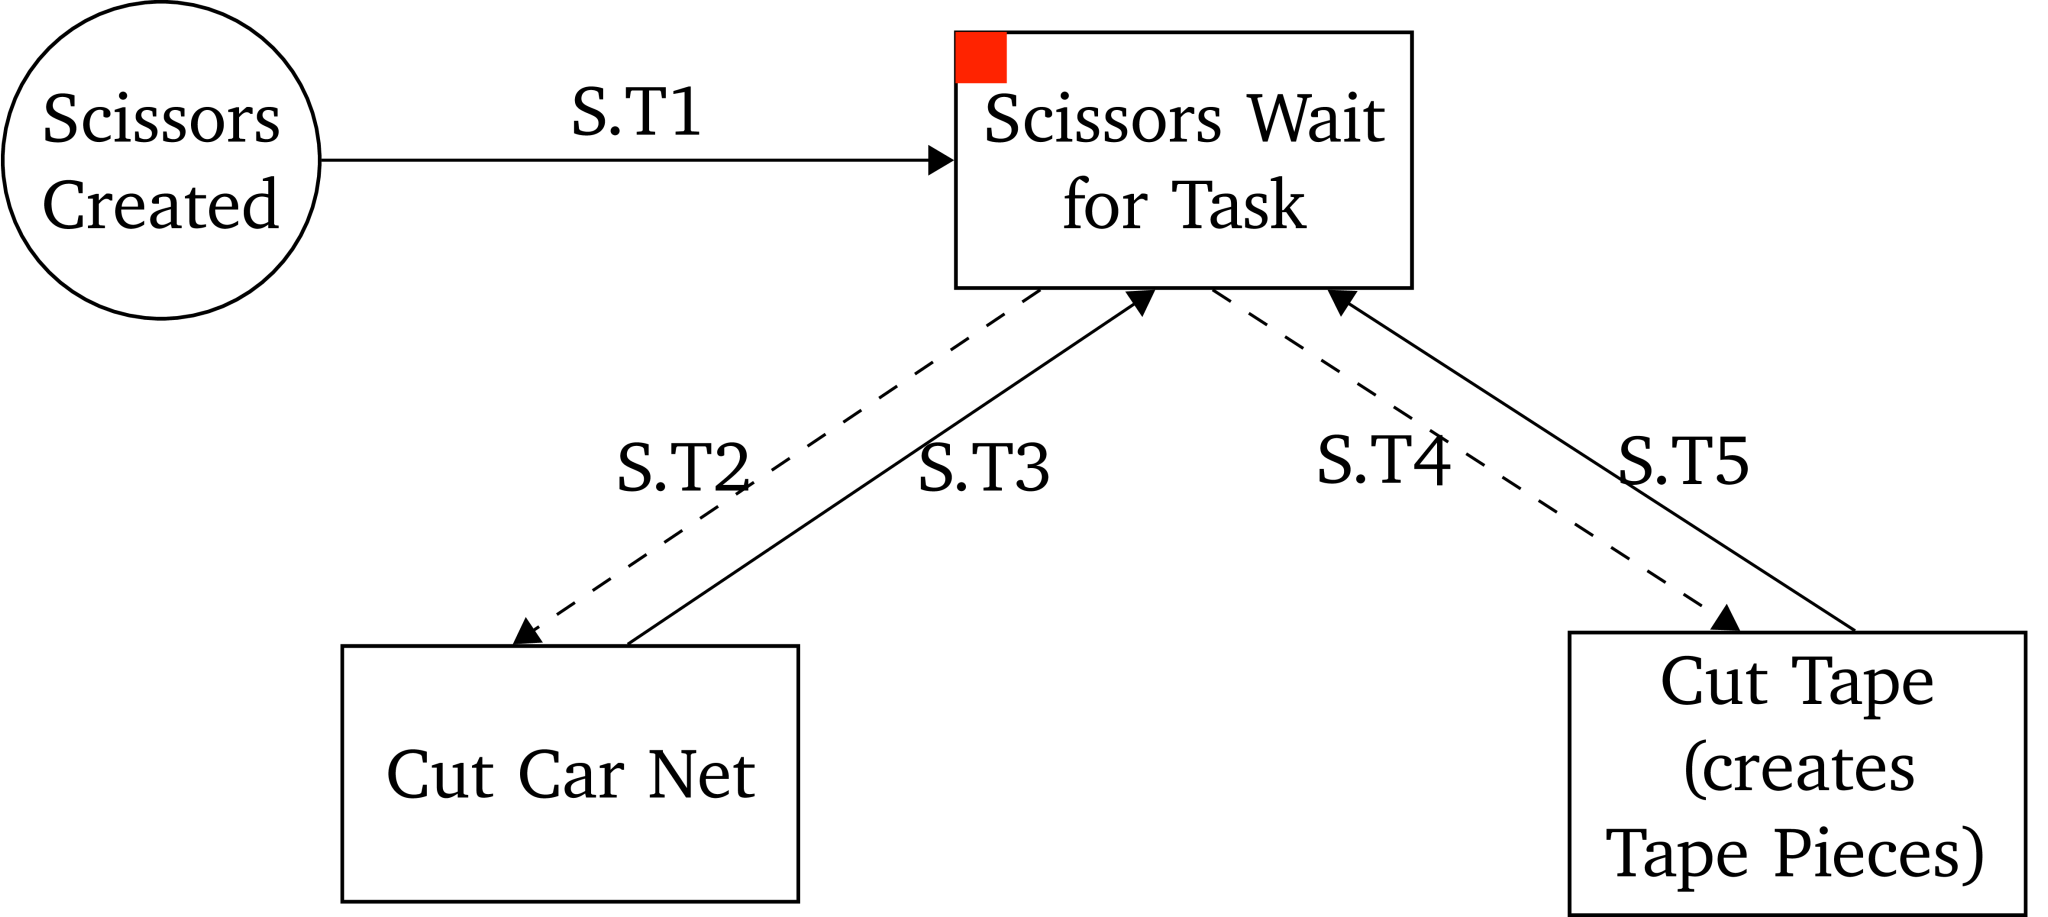
\includegraphics[width=100mm,height=\textheight]{chapters/cm_io_behaviour/figures/scissors-activity.pdf}

}

\caption{\label{fig-scissors_act}Scissors Activity Diagram}

\end{figure}%

\newpage{}

In the boxes below draw the activity diagrams for the remaining
entities.

\begin{figure*}

\begin{mdframed}[innerbottommargin=8cm]
~

~

~

~

~

~

~

~

~

~

~

~

~

~

~

~

~

~

~

~

~

~

~

~

~

~

\end{mdframed}

\end{figure*}%

~

\begin{figure*}

\begin{mdframed}[innerbottommargin=5cm]
~

~

~

~

~

~

~

~

~

~

~

~

~

\end{mdframed}

\end{figure*}%

~

\begin{figure*}

\begin{mdframed}[innerbottommargin=5cm]
~

~

~

~

~

~

~

~

~

~

~

~

~

\end{mdframed}

\end{figure*}%

~

\begin{figure*}

\begin{mdframed}[innerbottommargin=7cm]
~

~

~

~

~

~

~

~

~

~

~

~

~

~

~

~

\end{mdframed}

\end{figure*}%

\chapter{Data, Structure, and Logic}\label{data-structure-and-logic}

In this lab you will complete the remainder of the fourth phase of the
HCCM framework, with your group.

\section{Define the Data}\label{define-the-data-1}

Firstly, you need to give detailed definitions of the data modules. You
may not have collected data during car making, but complete the
following table that describes the kind of data you would need to
collect to simulate car making. Also add a comment on how the entry for
CutTapeDuration would change if no person-by-person data was available,
but an Exponential distribution that estimated the time it takes for a
person to cut tape was available.

\begin{table*}

\caption{\label{tbl-data_pc}List of Data Modules}

\centering{

\begin{tabular}{llllll}
  \toprule
    Name & Source & Model & Type & Input & Output \\ \midrule
    NumPencils & System info & Constant & Deterministic & - & The number of pencils available \\
    NumScissors & System info & Constant & Deterministic & - & The number of scissors available \\
    NumTape & System info & Constant & Deterministic & - & The number of rolls of tape available \\
    Num & System info & Constant & Deterministic & - &  \\
     &  &  &  & &  \\
    TraceCar & Experimental data & Lookup & Deterministic & Person & Time to trace car \\
    CutNet & Experimental data & Lookup & Deterministic & Person & Time to cut the net out \\
    &  &  &  & &  \\
    &  &  &  & &  \\
    &  &  &  & &  \\
    &  &  &  & &  \\
    &  &  &  & &  \\
    &  &  &  & &  \\
    CutTape & Experimental data & Lookup & Deterministic & Person & Time to cut a piece of tape \\ \bottomrule
  \end{tabular}

}

\end{table*}%

\section{Define the Structure}\label{define-the-structure-1}

The first part of the structure to define is the entities.
Table~\ref{tbl-entities_pc} lists the entities again, but adds
attributes that the entities will need to capture the performance of the
system, e.g., waiting time until the cube was cut. It is assumed that
all entities have the three attributes: ID, CurrentActivity, and
CurrentStart. These are omitted in the table to prevent repitition.

\begin{table}

\caption{\label{tbl-entities_pc}List of Entities}

\centering{

\begin{tabular}{ll}
\toprule
Entity  & Attributes        \\ \midrule
Paper   & WaitForTrace[0.0]    \\
        & WaitForCutShape[0.0] \\
        & WaitForFold[0.0]     \\
        & WaitForTapeCube[0.0] \\
        &                      \\
Pencil  & WaitForTrace[0.0]    \\
        &                      \\
Scissors& WaitForTask[0.0]     \\
        &                      \\
Tape    & WaitForCut[0.0]      \\
        &                      \\
TapePieces  & WaitForTape[0.0] \\
        & ArrivalTime[0.0]     \\
        & LeavingTime[0.0]     \\
Person  & WaitForTask[0.0]     \\ \bottomrule
\end{tabular}

}

\end{table}%

The next part of the structure is the transitions, which describe how
entities move between activites and events.
Table~\ref{tbl-transitions_pc} lists the transitions for making paper
cars. These transitions are prefixed by entity of the behavioural
pathway they come from. Complete the transitions for the Scissors
pathway.

\begin{table*}[H]

\caption{\label{tbl-transitions_pc}List of Transitions}

\centering{

\begin{tabular}{p{2.4cm}>{\raggedright\arraybackslash}p{1.2cm}>{\raggedright\arraybackslash}p{5.9cm}>{\raggedright\arraybackslash}p{5.9cm}}
\toprule
Participant & Name & From Event & To Event       \\ \midrule
Paper & PAP.1 & Paper Created & Paper Wait for Trace.Start \\
      & PAP.2 & Paper Wait for Trace.End & Trace Car.Start \\
      & PAP.3 & Trace Car.End & Paper Wait for Cut Net.Start \\
      & PAP.4 & Paper Wait for Cut Net.End & Cut Car Net.Start \\
      & PAP.5 & Cut Car Net.End & Car Wait for Fold.Start \\
      & PAP.6 & Car Wait for Fold.End & Fold Car.Start \\
      & PAP.7 & Fold Car.End & Car Wait for Tape.Start \\
      & PAP.8 & Car Wait for Tape.End & Tape Car.Start \\
      & PAP.9 & Tape Car.End & Car Finished \\
      &      &              &              \\
Pencil & PEN.1 & Pencil/Template Created & Pencil Wait for Trace.Start \\
       & PEN.2 & Pencil Wait for Trace.End & Trace Car.Start \\
       & PEN.3 & Trace Car.End & Pencil Wait for Trace.Start \\
       &      &              &              \\
Scissors & S.1 & Scissors Created             &              \\
       & S.2   &              &              \\
       & S.3   &              &              \\
       & S.4   &              &              \\
       & S.5   &              &              \\
       &      &              &              \\
Tape   & T.1 & Tape Created & Tape Wait for Cut.Start \\
       & T.2 & Tape Wait for Cut.End & Cut Tape.Start \\
       & T.3 & Cut Tape.End & Tape Wait for Cut.Start \\
       &      &              &              \\
Tape Piece & TP.1 & Tape Pieces Created & Tape Pieces Wait for Tape.Start \\
           & TP.2 & Tape Pieces Wait for Tape.End & Tape Car.Start \\
           & TP.3 & Tape Car.End & Tape Pieces Leave \\
     &      &              &              \\
Person & PER.1 & Person Created & Person Wait for Task.Start \\
       & PER.2 & Person Wait for Task.End & Trace Car.Start \\
       & PER.3 & Trace Car.End & Person Wait for Task.Start \\
       & PER.4 & Person Wait for Task.End & Cut Car Net.Start \\
       & PER.5 & Cut Car Net.End & Person Wait for Task.Start \\
       & PER.6 & Person Wait for Task.End & Fold Car.Start \\
       & PER.7 & Fold Car.End & Person Wait for Task.Start \\
       & PER.8 & Person Wait for Task.End & Cut Tape.Start \\
       & PER.9 & Cut Tape.End & Person Wait for Task.Start \\
       & PER.10 & Person Wait for Task.End & Tape Car.Start \\
       & PER.11 & Tape Car.End & Person Wait for Task.Start \\\bottomrule
\end{tabular}

}

\end{table*}%

\begin{longtable}{@{}>{\raggedright\arraybackslash}p{1.8cm}>{\raggedright\arraybackslash}p{2.1cm}>{\raggedright\arraybackslash}p{0.9cm}>{\raggedright\arraybackslash}p{2.2cm}>{\raggedright\arraybackslash}p{8.75cm}@{}}

\caption{\label{tbl-activities_pc}Activities}

\tabularnewline

  \toprule
  Activity                                   & Participants                                             & Event & Type       & State Change \\ \midrule
  \endhead
  Paper Wait for Trace      & Paper (P)                            & Start & Scheduled  & 
\begin{lstlisting}[language=CMPseudo]
(Default, omitted hereafter) P.CurrentActivity = "this activity"
(Default, omitted hereafter) P.CurrentStart = TIME
TRIGGER OnStartPaperWaitForTrace WITH C
\end{lstlisting}             \\
                                             &                                                          & End   & Controlled &
  \begin{lstlisting}[language=CMPseudo]
P.WaitForTrace = TIME - P.CurrentStart
# TRANSITION PAP.2 in logic
  \end{lstlisting}              \\ \midrule
  Trace Car                 & Paper (P), Person (H), Pencil (N)       & Start & Controlled &  
\begin{lstlisting}[language=CMPseudo]
SCHEDULE END at TIME + TraceCube(H)
\end{lstlisting}              \\
                                             &                                                          & End   & Scheduled  & 
\begin{lstlisting}[language=CMPseudo]
START Paper Wait for Cut Net WITH P # TRANSITION PAP.3
START Person Wait for Task WITH H # TRANSITION PER.3
START Pencil Wait for Trace WITH N # TRANSITION PEN.3
\end{lstlisting}              \\ \midrule
  Paper Wait for Cut Net    &                                & Start &   & 
\begin{lstlisting}[language=CMPseudo]
TRIGGER OnStartPaperWaitForCutNet WITH P
\end{lstlisting}              \\
  &                                                          & End   &  & 
\begin{lstlisting}[language=CMPseudo]
P.WaitForCutNet = TIME - P.CurrentStart
# TRANSITION PAP.4 in logic
\end{lstlisting}             \\ \midrule
  Cut Car Net               & Paper (P), Person (H), Scissors (S)     & Start & Controlled  & 
\begin{lstlisting}[language=CMPseudo]
SCHEDULE END at TIME + CutNet(H)
\end{lstlisting}             \\
  &                                                          & End   & Scheduled &
\begin{lstlisting}[language=CMPseudo]
START Car Wait for Fold WITH P # TRANSITION PAP.5
START Person Wait for Task WITH H # TRANSITION PER.5
START Scissors Wait for Task WITH S # TRANSITION S.3
\end{lstlisting}              \\ \midrule
  Car Wait for Fold         & Paper (P)                              & Start & Scheduled  & 
\begin{lstlisting}[language=CMPseudo]
TRIGGER OnStartCarWaitForFold WITH P
\end{lstlisting}             \\
  &                                                          & End   & Controlled & 
\begin{lstlisting}[language=CMPseudo]
P.WaitForFold = TIME - P.CurrentStart
# TRANSITION PAP.6 in logic
\end{lstlisting}             \\ \midrule
  Fold Car                  & Paper (P), Person (H)                  & Start & Controlled  & 
\begin{lstlisting}[language=CMPseudo]
SCHEDULE END at TIME + FoldCar(H)
\end{lstlisting}             \\
  &                                                          & End   & Scheduled & 
\begin{lstlisting}[language=CMPseudo]
START Car Wait for Tape Car WITH P # TRANSITION PAP.7
START Person Wait for Task WITH H # TRANSITION PER.7
\end{lstlisting}             \\ \midrule
  \textcolor{red}{Car Wait for Tape Car}     &                                & Start &   & 
\begin{lstlisting}[language=CMPseudo]
 
\end{lstlisting}             \\
  &                                                          & End   &  & 
\begin{lstlisting}[language=CMPseudo]
 
 
\end{lstlisting}             \\ \midrule
  \textcolor{red}{Tape Car}                  &  & Start &   & 
\begin{lstlisting}[language=CMPseudo]
 
\end{lstlisting}             \\
  &                                                          & End   &  &
\begin{lstlisting}[language=CMPseudo]
 
 
 
\end{lstlisting}              \\ \midrule
  Pencil Wait for Trace    & Pencil (N)                             & Start & Scheduled  & 
\begin{lstlisting}[language=CMPseudo]
TRIGGER OnStartPencilWaitForTrace WITH N
\end{lstlisting}             \\
  &                                                          & End   & Controlled & 
\begin{lstlisting}[language=CMPseudo]
N.WaitForTrace = N.WaitForTrace + TIME - N.CurrentStart
# TRANSITION N.2 in logic
\end{lstlisting}             \\ \midrule
  Scissors Wait for Task    & Scissors (S)                            & Start & Scheduled  & 
\begin{lstlisting}[language=CMPseudo]
TRIGGER OnStartScissorsWaitForTask WITH S
\end{lstlisting}             \\
  &                                                          & End   & Controlled & 
\begin{lstlisting}[language=CMPseudo]
S.WaitForTask = S.WaitForTask + TIME - S.CurrentStart
# TRANSITION S.2 or S.4 in logic
\end{lstlisting}             \\ \midrule
  Cut Tape                  & Tape (T), Person (H), Scissors (S)      & Start & Controlled  & 
\begin{lstlisting}[language=CMPseudo]
SCHEDULE END at TIME + CutTape(H)
\end{lstlisting}             \\
  &                                                          & End   & Scheduled & 
\begin{lstlisting}[language=CMPseudo]
START Person Wait for Task WITH H # TRANSITION PER.9
START Scissors Wait for Task WITH S # TRANSITION S.5
START Tape Wait for Cut WITH T # TRANSITION T.3
CREATE Tape Pieces TP
START Tape Pieces Created WITH TP
\end{lstlisting}             \\ \midrule
  Tape Wait for Cut         & Tape (T)                                & Start & Scheduled  & 
\begin{lstlisting}[language=CMPseudo]
TRIGGER OnStartTapeWaitForCut WITH T
\end{lstlisting}             \\
  &                                                          & End   & Controlled & 
\begin{lstlisting}[language=CMPseudo]
T.WaitForCut = T.WaitForCut + TIME - T.CurrentStart
# TRANSITION T.2 in logic
\end{lstlisting}             \\ \midrule
  Tape Pieces Wait for Tape & Tape Pieces (TP)                       & Start & Scheduled  & 
\begin{lstlisting}[language=CMPseudo]
TRIGGER OnStartTapePiecesWaitForTape WITH TP
\end{lstlisting}             \\
  &                                                          & End   & Controlled & 
\begin{lstlisting}[language=CMPseudo]
TP.WaitForTape = TP.WaitForTape + TIME - TP.CurrentStart
# TRANSITION TP.2 in logic
\end{lstlisting}             \\ \midrule
  \textcolor{red}{Person Wait for Task}      &                              & Start &   & 
\begin{lstlisting}[language=CMPseudo]
 
\end{lstlisting}             \\
  &                                                          & End   &  & 
\begin{lstlisting}[language=CMPseudo]
 
 
\end{lstlisting}             \\ \bottomrule
  

\end{longtable}

\part{Jaamsim Labs}

\chapter{Using Traces and Scenarios}\label{using-traces-and-scenarios}

In this lab we will modify the simulation developed in the previous lab
to run off of a pre-generated data trace that contains information about
each patient. We will also explore how Jaamsim's built-in scenario
indices can be used to run experiments where the values of the
simulation's inputs are changed and use an EventLogger to log all events
that an entity participates in. Finally we will package the simulation
(Jaamsim and the custom Java code) as a .jar file, so that the
simulation can be run easily from the command line on all major
operating systems.

We are not considering any changes to the system, so the conceptual
model is the same as for the previous lab.

\section{Jaamsim Model}\label{jaamsim-model}

To run the simulation from a data trace we need to make some changes to
the Jaamsim model. Once again create a new folder called \textbf{RC3}
and copy your .cfg file (and the .png files so that the graphics work)
from the previous lab folder into this folder and rename it to
\textbf{radiology\_lab\_trace.cfg}. First, download the
\textbf{RC\_50\_week\_data.txt} file from Canvas. This file contains 50
weeks of data of patients at the radiology clinic including: the time
the patient arrived, the priority of the patient, the time the patient
took to check in, and the time the patient took to have their scan.

Before we load the data in we will first change the starting date of the
simulation, which defaults to 1970, to instead be 2024, so that the data
read from the file is interpreted correctly. To do this go to the
Simulation object and under the Options tab enter \textbf{2024-01-01}
for the StartDate.

To use the data in Jaamsim we use a \textbf{FileToMatrix} object found
in the Basic Objects palette. Create a FileToMatrixObject, rename it
\textbf{PatientData}, and select the \textbf{RC\_50\_-week\_data.txt}
file as the DataFile.

We can now access the data in the file by using the \textbf{Value}
output of the PatientData object. The first place we will use this data
is in the PatientArrival object, so that patients arrive according to
the data in the file, rather than the distribution used previously. We
first create two CustomOutputs (under the options tab) on the
PatientArrival object to make accessing the data easier. CustomOutputs
are similar to attributes but they can be expressions (formulas) and are
re-calculated at each time step in the simulation. The two outputs we
create will correspond to the data for the patient that has just arrived
(thisPatientData) and the patient that is going to arrive next
(nextPatientData). We need both of these so that we can calculate the
appropriate interarrival time between the patients.

Once we have created these outputs we use them in the InterArrivalTime,
and AssignmentList of the PatientArrival.

\begin{table*}[H]

\caption{\label{tbl-pat_arr}Update PatientArrival}

\centering{

\begin{tabular}{@{}lll@{}}
\toprule
Object            & Keyword         & Value         \\ \midrule
PatientArrival  & CustomOutputList & \{ thisPatientData  `[PatientData].Value(this.NumberAdded + 1)' \}\\
 & & \{ nextPatientData  `[PatientData].Value(this.NumberAdded + 2)' \}\\
                                 & FirstArrivalTime & [PatientData].Value(2)(2)\\
                                 & InterArrivalTime & `this.nextPatientData(2) - this.thisPatientData(2)'\\
                                 & AssignmentList & \{ `this.obj.priority= this.thisPatientData(3)' \} \\
 & & \{ `this.obj.checkInTime= this.thisPatientData(4)' \}
 \\ & & \{ `this.obj.scanTime= this.thisPatientData(5)' \}\\
\bottomrule
\end{tabular}

}

\end{table*}%

Note that in the AssignmentList we are assigning values from the data
file to attributes on the patient entity for priority, check in time,
and scan time. We will use these attributes later to determine how long
those activities take (the priority attribute is already used in the
PriorityBranch).

To avoid getting an error these attributes need to be added to the
PatientEntity object. So update the AttributeDefinitionList of the
PatientEntity to include checkInTime and scanTime as well as the current
priority, all with a default of 0.

We now need to use the checkInTime and scanTime attributes to determine
how long the check ins and scans take. Set the Duration of the CheckIn
activity to \textbf{this.CurrentParti-cipants(1).checkInTime *
1{[}min{]}}. this.CurrentParticipants refers to the group of entities
that have just started the activity (for check in this is a patient and
a receptionist), and we use the index 1 as the patient comes first, then
we access the checkInTime attribute. We then need to multiply this by
1{[}min{]} to convert the number into a time, and use minutes as the
attribute is in minutes.

Similarly for the Scan activity set the Duration to
\textbf{this.CurrentParticipants(1).scanTime * 1{[}h{]}}, note that here
we use 1{[}h{]} as the attribute is in hours.

Now, suppose we are interested in the time that patients spend waiting
for check in and for the scan. We can't use the current PatientLogger as
it only records the total time that patients are in the system for. We
could add attributes for each time that we are interested in, and assign
the value when the entity gets to the relevant stage, and then use the
PatientLogger to log these attributes. We can instead use an EventLogger
from the HCCM palette. The EventLogger records the time that an entity
starts each of the activities that it participates in. So, create an
EventLogger and call it PatientEventLogger.

Then, to get the events recorded go to the PatientLeave object and under
the HCCM tab enter PatientEventLogger for the EventLogger keyword. Now
any entities that are sent to the patient leave will have the start
times of any activities that they participated in recorded.

We will now configure the Simulation object to run one long replication
for several scenarios. Under the Key Inputs tab enter \textbf{50w} for
the \textbf{RunDuration}, this will make the simulation run for 50
weeks. We have to run one 50 week replication rather than 50 one week
replications as Jaamsim cannot read in a new file when each replication
starts.

We want to try out four scenarios with either three or four CT machines,
and either one or two receptionists. As there are two factors we are
changing we use a ScenarioIndex with two numbers, the first indexes the
scenarios relating to the number of CT Machines, and the second those
related to the number of receptionists.

Since there are two options for the first index and two for the second
we enter \textbf{2 2} for the \textbf{ScenarioIndexDefinitionList} under
the \textbf{MultipleRuns} tab of the \textbf{Simulation} object. We will
start from scenario 1 and end at scenario 2 in both the indices so
StartingScenarioNumber is \textbf{1-1} and EndingScenarioNumber is
\textbf{2-2}. We are going to run just one long replication for each
scenario so set the NumberOfReplications to 1.

Now Jaamsim will run 4 scenarios, but we need to make it so that the
number of CT Machines and Receptionists actually changes in each of the
scenarios. For the CT Machines we set the \textbf{MaxNumber} on the
\textbf{CTMachineArrival} to \textbf{{[}Simulation{]}.ScenarioIndex(1) +
2}, which gets the value of the first scenario index and adds 2 to it.
For the Receptionists we can set the \textbf{MaxNumber} on the
\textbf{ReceptionistArrival} to
\textbf{{[}Simulation{]}.ScenarioIndex(2)}, in this case we don't need
to add one as the scenario index is the same as the number of
receptionists we want to use.

Download and run the \textbf{RadiologyLabTraceAnalysis.R} file, you will
have to update the directory that it reads the data from and the name of
the data file used. The script splits each replication into 50 batches,
each one week long, and calculates the mean across the batches and the
four scenarios of the 90th percentile waiting time for both check in and
scan within each of batch. No warm-up period is used, so this assumes
that being empty and idle is a typical state of the system. Splitting
into batches by week assumes that each week is not correlated to the
preceding and following weeks. You should get the following output:

\part{Conceptual Models}

\chapter{Radiology Clinic}\label{sec-radiology_cm}

\section{Data}\label{data}

\begin{table*}

\caption{\label{tbl-var_lab1}List of Global Variables}

\centering{

\begin{tabular}{p{4cm}p{4cm}p{2cm}}
  \toprule
  Name    & Description & Initial Value        \\ \midrule
  NextPatIdNum & The Id number that will be assigned to the next patient & 1 \\
  NextReceptionistIdNum & The Id number that will be assigned to the next receptionist & 1 \\
  NextCTMachineIdNum & The Id number that will be assigned to the next CT Machine & 1 \\ 
  $P$ & The set of all patients & $\emptyset$ \\
  $R$ & The set of all receptionists & $\emptyset$ \\
  $C$ & The set of all CT Machines & $\emptyset$ \\ \bottomrule
\end{tabular}

}

\end{table*}%

\begin{table*}

\caption{\label{tbl-data_lab1}List of Data Modules}

\centering{

\begin{tabular}{lllll}
\toprule
  Name             & Source                                                            & Identification & Input                                                            & Output                                                             \\ \midrule
  PatientInterarrivalTime & Poisson Process         & Parameter      & Mean interarrival time & Sample from Distribution \\
  NumReceptionists        & Constant                                                          & Parameter      & N/A                                                              & Value                                                              \\
  NumCTMachines           & Constant                                                          & Parameter      & N/A                                                              & Value                                                              \\
  CheckInTime             & Uniform Distribution    & Parameter      & Min and max time       & Sample from Distribution \\
  ScanTime                & Log-normal Distribution & Parameter      & Mean and std. dev.     & Sample from Distribution \\ \bottomrule
\end{tabular}

}

\end{table*}%

\newpage{}

\section{Components}\label{components}

\begin{table*}

\caption{\label{tbl-entities_lab1}List of Entities}

\centering{

\begin{tabular}{ll}
\toprule
Entity  & Attributes        \\ \midrule
Patient & ID                \\
        & State             \\
        & StateTimes       \\
        &                   \\
Receptionist   & ID                \\
        & State             \\
        & StateTimes       \\
        &                   \\
CT Machine  & ID                \\
        & State             \\
        & StateTimes       \\ \bottomrule
\end{tabular}

}

\end{table*}%

\begin{table*}

\caption{\label{tbl-transitions_lab1}List of Transitions}

\centering{

\begin{tabular}{p{0.6cm}>{\raggedright\arraybackslash}p{2.4cm}>{\raggedright\arraybackslash}p{5.9cm}>{\raggedright\arraybackslash}p{5.9cm}}
\toprule
No. & Participant & From Event & To Event       \\ \midrule
1 & Patient  & Arrive(P) & Wait for check in.Start \\
2 & Patient & Wait for check in.End & Check in.Start\\
3 & Patient & Check in.End & Wait for scan.Start\\
4 & Patient & Wait for scan.End & Scan.Start\\
5 & Patient & Scan.End & Leave(P)\\
6 & Receptionist  & Arrive(R)& Wait for task(R).Start\\
7 & Receptionist  & Wait for task(R).End & Check in.Start\\
8 & Receptionist  & Check in.End & Wait for task(R).Start\\
9 & Receptionist  & Wait for task(R).End& Leave(R)\\
10& CT Machine  & Arrive(CT)& Wait for task(CT).Start\\
11& CT Machine  & Wait for task(CT).End & Scan.Start\\
12& CT Machine & Scan.End & Wait for task(CT).Start\\
13& CT Machine  & Wait for task(CT).End& Leave(CT)\\\bottomrule
\end{tabular}

}

\end{table*}%

\begin{longtable}{@{}>{\raggedright\arraybackslash}p{1.8cm}>{\raggedright\arraybackslash}p{2.1cm}>{\raggedright\arraybackslash}p{0.9cm}>{\raggedright\arraybackslash}p{2.2cm}>{\raggedright\arraybackslash}p{8cm}@{}}

\caption{\label{tbl-activities_lab1}Activities}

\tabularnewline

  \toprule
  Activity          & Participants & Event & Type       & State Change \\ \midrule
  \endhead
  Wait for Check In & Patient (p)  & Start & Scheduled  & 
  \vspace{-12pt}
  \begin{lstlisting}[language=CMPseudo]
TRIGGER OnStartWaitForCheckIn WITH p
  \end{lstlisting}
  \\[-12pt] \cmidrule{3-5}
                    &              & End   & Controlled &
  
  \\ \midrule
  Check In & Patient (p), Receptionist (r)  & Start & Controlled  & 
  \vspace{-12pt}
  \begin{lstlisting}[language=CMPseudo]
SCHEDULE Check In.End at TIME + CheckInTime()
  \end{lstlisting}
  \\[-12pt] \cmidrule{3-5}
                    &              & End   & Scheduled &
  \vspace{-12pt}
  \begin{lstlisting}[language=CMPseudo]
START Wait for Scan WITH p
START Wait for Task (R) WITH r
  \end{lstlisting}          
  \\[-12pt] \midrule
  Wait for Scan & Patient (p)  & Start & Scheduled  &              \\ \cmidrule{3-5}
                &              & End   & Controlled &
  \vspace{-12pt}
  \begin{lstlisting}[language=CMPseudo]
TRIGGER OnStartWaitForScan WITH p
  \end{lstlisting}
  \\[-12pt] \midrule
  Scan & Patient (p), CTMachine (c)  & Start & Controlled  & 
  \vspace{-12pt}
  \begin{lstlisting}[language=CMPseudo]
SCHEDULE Scan.End at TIME + ScanTime()
  \end{lstlisting}
  \\[-12pt] \cmidrule{3-5}
                    &              & End   & Scheduled &
  \vspace{-12pt}
  \begin{lstlisting}[language=CMPseudo]
START Leave (P) WITH p
START Wait for Task (CT) WITH c
  \end{lstlisting}          
  \\[-12pt] \midrule
  Wait for Task (R) & Receptionist (r)  & Start & Scheduled  &
  \vspace{-12pt}
  \begin{lstlisting}[language=CMPseudo]
TRIGGER OnStartWaitForTaskR WITH r
  \end{lstlisting}
  \\[-12pt] \cmidrule{3-5}
                    &              & End   & Controlled &
  
  \\ \midrule
  Wait for Task (CT) & CTMachine (c)  & Start & Scheduled  &
  \vspace{-12pt}
  \begin{lstlisting}[language=CMPseudo]
TRIGGER OnStartWaitForTaskCT WITH c
  \end{lstlisting}
  \\[-12pt] \cmidrule{3-5}
                    &              & End   & Controlled &
  \\ \bottomrule
  

\end{longtable}

\begin{longtable}{@{}>{\raggedright\arraybackslash}p{1.5cm}>{\raggedright\arraybackslash}p{2.1cm}>{\raggedright\arraybackslash}p{2.2cm}>{\raggedright\arraybackslash}p{10cm}@{}}

\caption{\label{tbl-events_lab1}Events}

\tabularnewline

  \toprule
  Activity          & Participants & Type       & State Change \\ \midrule
  \endhead
  Simulation Start & -  & Scheduled  & 
  \vspace{-12pt}
  \begin{lstlisting}[language=CMPseudo]
SCHEDULE Arrival (R) at TIME
SCHEDULE Arrival (CT) at TIME
SCHEDULE Arrival (P) at TIME + PatientInterArrival()
  \end{lstlisting}
  \\ \midrule
  Arrival (P) & Patient (p)  & Scheduled  & 
  \vspace{-12pt}
  \begin{lstlisting}[language=CMPseudo]
p.ID = NextPatIDNum
p.Priority = PatientPriority()
NextPatIDNum = NextPatIDNum + 1
SCHEDULE Arrival (P) at TIME + PatientInterArrival()
START Wait for Check In WITH p
  \end{lstlisting}
  \\ \midrule
  Leave (P) & Patient (p)  & Scheduled  & 
  \vspace{-12pt}
  \begin{lstlisting}[language=CMPseudo]
Calculate statistics for p
  \end{lstlisting}
  \\ \midrule
  Arrival (R) & Receptionist (r)  & Scheduled  & 
  \vspace{-12pt}
  \begin{lstlisting}[language=CMPseudo]
r.ID = NextReceptionistIDNum
NextReceptionistIDNum = NextReceptionistIDNum + 1
IF NextReceptionistIDNum <= NumReceptionists THEN
    SCHEDULE Arrival (R) at TIME
END IF
START Wait for Task (R) WITH r
  \end{lstlisting}
  \\ \midrule
  Leave (R) & Receptionist (r)  & Scheduled  & 
  \vspace{-12pt}
  \begin{lstlisting}[language=CMPseudo]
Calculate statistics for r
  \end{lstlisting}
  \\ \midrule
  Arrival (CT) & CTMachine (c)  & Scheduled  & 
  \vspace{-12pt}
  \begin{lstlisting}[language=CMPseudo]
c.ID = NextCTMachineIDNum
NextCTMachineIDNum = NextCTMachineIDNum + 1
IF NextCTMachineIDNum <= NumCTMachines THEN
    SCHEDULE Arrival (CT) at TIME
END IF
START Wait for Task (CT) WITH c
  \end{lstlisting}
  \\ \midrule
  Leave (P) & CTMachine (c)  & Scheduled  & 
  \vspace{-12pt}
  \begin{lstlisting}[language=CMPseudo]
Calculate statistics for c
  \end{lstlisting}
  \\ \bottomrule
  

\end{longtable}

\newpage{}

\section{Activity Diagrams}\label{activity-diagrams}

\begin{figure}[htbp]

\centering{

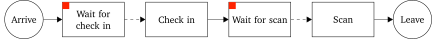
\includegraphics[width=155mm,height=\textheight]{chapters/clinic_1_cm/figures/patient_activity.pdf}

}

\caption{\label{fig-pat_act}Patient Activity Diagram}

\end{figure}%

\begin{figure}[htbp]

\centering{

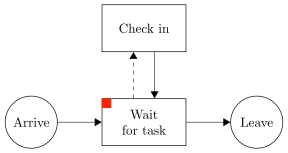
\includegraphics[width=76mm,height=\textheight]{chapters/clinic_1_cm/figures/receptionist_activity.pdf}

}

\caption{\label{fig-recep_act}Receptionist Activity Diagram}

\end{figure}%

\begin{figure}[htbp]

\centering{

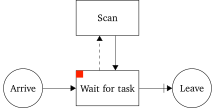
\includegraphics[width=76mm,height=\textheight]{chapters/clinic_1_cm/figures/CT_activity.pdf}

}

\caption{\label{fig-ct_act}CT Activity Diagram}

\end{figure}%

\newpage{}

\section{Control Policies}\label{control-policies}

\begin{table*}

\caption{\label{tbl-start_wait_check_in}OnStartWaitForCheckIn}

\centering{

\begin{tabular}{@{}>{\raggedright\arraybackslash}p{0.25cm}>{\raggedright\arraybackslash}p{13cm}@{}}
  \toprule
   & Triggered by: Patient p\\ \midrule 
  &
\vspace{-12pt}
\begin{lstlisting}[language=CMPseudo]
receps = {r FOR r IN R IF r.State = "Wait for task (R)"}
IF receps IS NOT empty THEN 
    r_hat = argmin{r.CurrentStart FOR r IN receps}
    START Check In WITH p, r_hat
END IF
\end{lstlisting}
  \\ \bottomrule
  \end{tabular}

}

\end{table*}%

\begin{table*}

\caption{\label{tbl-start_wait_check_in}OnStartWaitForScan}

\centering{

\begin{tabular}{@{}>{\raggedright\arraybackslash}p{0.25cm}>{\raggedright\arraybackslash}p{13cm}@{}}
  \toprule
   & Triggered by: Patient p\\ \midrule 
  &
\vspace{-12pt}
\begin{lstlisting}[language=CMPseudo]
cts = {c FOR c IN C IF c.State = "Wait for task (C)"}
IF cts IS NOT empty THEN 
    c_hat = argmin{c.CurrentStart FOR c IN cts}
    START Scan WITH p, r_hat
END IF
  \end{lstlisting}
  \\[-12pt] \bottomrule
  \end{tabular}

}

\end{table*}%

\begin{table*}

\caption{\label{tbl-start_wait_check_in}OnStartWaitForTaskR}

\centering{

\begin{tabular}{@{}>{\raggedright\arraybackslash}p{0.25cm}>{\raggedright\arraybackslash}p{13cm}@{}}
  \toprule
   & Triggered by: Receptionist r\\ \midrule 
  &
\vspace{-12pt}
\begin{lstlisting}[language=CMPseudo]
patients = {p FOR p IN P IF p.State = "Wait for Check In"}
IF patients IS NOT empty THEN 
    p_hat = argmin{p.CurrentStart FOR p IN patients}
    START Check In WITH p, r_hat
END IF
  \end{lstlisting}  
  \\[-12pt] \bottomrule
  \end{tabular}

}

\end{table*}%

\begin{table*}

\caption{\label{tbl-start_wait_check_in}OnStartWaitForTaskCT}

\centering{

\begin{tabular}{@{}>{\raggedright\arraybackslash}p{0.25cm}>{\raggedright\arraybackslash}p{13cm}@{}}
  \toprule
   & Triggered by: CTMachine c\\ \midrule 
  &
\vspace{-12pt}
\begin{lstlisting}[language=CMPseudo]
patients = {p FOR p IN P IF p.State = "Wait for Scan"}
IF patients IS NOT empty THEN 
    p_hat = argmin{p.CurrentStart FOR p IN patients}
    START Scan WITH p, r_hat
END IF
  \end{lstlisting}
  \\[-12pt] \bottomrule
  \end{tabular}

}

\end{table*}%




\end{document}
